\documentclass[12pt]{article}
\usepackage[paper=letterpaper,margin=2cm]{geometry}
\usepackage{amsmath,amssymb,amsfonts}
\usepackage{enumitem}
\usepackage{titling}
\usepackage{multirow}
\usepackage{xcolor}
\usepackage{float}
\usepackage{graphicx}
\usepackage{xcolor}
\definecolor{ISTBlue}{RGB}{0, 139, 255}
\usepackage[colorlinks=true, linkcolor=red]{hyperref}
\usepackage{subcaption} % For subfigures
\usepackage{adjustbox}  % For centering the bottom image
\usepackage{listings}
\usepackage{xcolor} % para personalizar as cores (opcional)

\usepackage{listings}
\usepackage{xcolor}

\definecolor{codegreen}{rgb}{0.0, 0.514, 0.325}      
\definecolor{codegray}{rgb}{0.75, 0.75, 0.75}    
\definecolor{codeblue}{rgb}{0.122, 0.467, 0.706}  
\definecolor{extraLightGray}{rgb}{0.98, 0.98, 0.98}
\definecolor{codepink}{rgb}{0.894, 0.0, 0.443}

\lstdefinestyle{mystyle}{
    backgroundcolor=\color{extraLightGray},
    commentstyle=\color{codegreen},
    keywordstyle=\color{codeblue},
    numberstyle=\tiny\color{codegray},
    stringstyle=\color{codepink},
    basicstyle=\ttfamily\footnotesize,
    breakatwhitespace=false,
    breaklines=true,
    captionpos=b,
    keepspaces=true,
    numbers=left,
    numbersep=5pt,
    showspaces=false,
    showstringspaces=false,
    showtabs=false,
    tabsize=2
}
\lstset{style=mystyle}

\setlength{\droptitle}{-6em}

\begin{document}

\begin{center}
Aprendizagem 2023\\
Homework I --- Group 003\\
(ist1107028, ist1107137)\vskip 1cm
\end{center}

\large{\textbf{Part I}: Pen and paper}\normalsize

\begin{enumerate}[leftmargin=\labelsep]
\item \textbf{Complete the given decision tree using Shannon entropy ($\log_2$) and considering that:
    (i) a minimum of 4 observations is required to split an internal node, and (ii) decisions by ascending alphabetic should be placed in case of ties.}

\vspace{1em}
The entropy of $y_\text{out}$ is given by:

\begin{equation*}
    \begin{split}
        H(y_{\text{out}}|y_1 >= 0.3) = &- P(y_{\text{out}} = A|y_1 >= 0.3)\log_2(P(y_{\text{out}} = A|y_1 >= 0.3)) \\
        &- P(y_{\text{out}} = B|y_1 >= 0.3)\log_2(P(y_{\text{out}} = B|y_1 >= 0.3)) \\
        &- P(y_{\text{out}} = C|y_1 >= 0.3)\log_2(P(y_{\text{out}} = C|y_1 >= 0.3)) \\
    \end{split}
\end{equation*}

Replacing by the values is obtained:

\begin{equation*}
    H(y_{\text{out}}|y_1 >= 0.3) = - \left( \frac{3}{7} \log_2 \left( \frac{3}{7} \right) + \frac{2}{7} \log_2 \left( \frac{2}{7} \right) + \frac{2}{7} \log_2 \left( \frac{2}{7} \right) \right) \approx  1.5567
\end{equation*}

\vspace{0.5em}
We must now calculate $H(y_{\text{out}} | y_1 >= 0.3, y_x)$, in which x will assume the values of 2, 3 and 4:

\begin{equation}
    \label{H-y_out}
    \begin{split}
    H(y_{\text{out}} | y_1 >= 0.3, y_x) = P(y_x = 0 | y_1 >= 0.3) H(y_{\text{out}} | y_1 >= 0.3, y_x = 0) \\
    + P(y_x = 1 | y_1 >= 0.3) H(y_{\text{out}} | y_1 >= 0.3, y_x = 1) \\
    + P(y_x = 2 | y_1 >= 0.3) H(y_{\text{out}} | y_1 >= 0.3, y_x = 2)
    \end{split}
\end{equation}

The information gain of $y_x$ is given by:

\begin{equation}\label{IG}
    IG(y_{\text{out}} | y_1 >= 0.3, y_x) = H(y_{\text{out}} | y_1 >= 0.3) - H(y_{\text{out}} | y_1 >= 0.3, y_x)
\end{equation}

\vspace{0.2cm}
\fbox{x=2:}

\begin{equation*}
    P(y_2 = 0 | y_1 >= 0.3) = \frac{4}{7} \quad
    P(y_2 = 1 | y_1 >= 0.3) = \frac{3}{7} \quad
    P(y_2 = 2 | y_1 >= 0.3) = \frac{0}{7} \quad
\end{equation*}

\begin{equation*}
    \begin{aligned}
        H(y_{\text{out}} | y_1 >= 0.3, y_2 = 0) &= - \left( \frac{1}{4} \log_2 \left( \frac{1}{4} \right) + \frac{1}{4} \log_2 \left( \frac{1}{4} \right) + \frac{2}{4} \log_2 \left( \frac{2}{4} \right) \right) = 1.5
        \\
        H(y_{\text{out}} | y_1 >= 0.3, y_2 = 1) &= - \left( \frac{2}{3} \log_2 \left( \frac{2}{3} \right) + \frac{1}{3} \log_2 \left( \frac{1}{3} \right) + \frac{0}{3} \log_2 \left( \frac{0}{3} \right) \right) \approx 0.9183
        \\
    \end{aligned}
\end{equation*}

\newpage

\begin{flushleft}
    On account of the fact that $P(y_2 = 2 | y_1 >= 0.3) = \frac{0}{7} = 0$, $H(y_{\text{out}} | y_1 >= 0.3, y_2 = 2)$ will also be 0.\\
    \vspace{1em}
    Thus, by inserting these values into equation~\eqref{H-y_out}, we get:
\end{flushleft}

\begin{equation*}
    H(y_{\text{out}} | y_1 >= 0.3, y_2) = \frac{4}{7} \times 1.5 + \frac{3}{7} \times 0.9183 + \frac{0}{7} \times 0 = 1.2507
    \\
\end{equation*}
\\
Lastly, we calculate the information gain as per~\eqref{IG}:

\begin{equation*}
    IG(y_{\text{out}} | y_1 >= 0.3, y_2) = 1.5567 - 1.2507 = 0.306
\end{equation*}

\fbox{x=3:}
\begin{equation*}
    P(y_3 = 0|y_1 >= 0.3) = \frac{2}{7} \quad
    P(y_3 = 1|y_1 >= 0.3) = \frac{4}{7} \quad
    P(y_3 = 2|y_1 >= 0.3) = \frac{1}{7} \quad
\end{equation*}

\begin{equation*}
    \begin{aligned}
        H(y_{\text{out}}|y_1 >= 0.3, y_3 = 0) = - \left( \frac{2}{2} \log_2 \left( \frac{2}{2} \right) + \frac{0}{2} \log_2 \left( \frac{0}{2} \right) + \frac{0}{2} \log_2 \left( \frac{0}{2} \right) \right) &= 0 
        \\
        H(y_{\text{out}}|y_1 >= 0.3, y_3 = 1) = - \left( \frac{1}{4} \log_2 \left( \frac{1}{4} \right) + \frac{1}{4} \log_2 \left( \frac{1}{4} \right) + \frac{2}{4} \log_2 \left( \frac{2}{4} \right) \right) &= 1.5
        \\
        H(y_{\text{out}}|y_1 >= 0.3, y_3 = 2) = - \left( \frac{0}{1} \log_2 \left( \frac{0}{1} \right) + \frac{1}{1} \log_2 \left( \frac{1}{1} \right) + \frac{0}{1} \log_2 \left( \frac{0}{1} \right) \right) &= 0
    \end{aligned}
\end{equation*}

Thus, by inserting these values into equation~\eqref{H-y_out}, we get:

\begin{equation*}
    H(y_{\text{out}}|y_1 >= 0.3, y_3) = \frac{2}{7} \times  0 + \frac{4}{7} \times 1.5 + \frac{1}{7} \times 0 \approx 0.8571 
\end{equation*}
\\
Lastly, we calculate the information gain as per~\eqref{IG}:

\begin{equation*}
    IG(y_{\text{out}} | y_1 >= 0.3, y_3) = 1.5567 - 0.8571 = \textbf{0.6996}
\end{equation*}

\fbox{x=4:}
\begin{equation*}
    P(y_4 = 0|y_1 >= 0.3) = \frac{4}{7} \quad
    P(y_4 = 1|y_1 >= 0.3) = \frac{3}{7} \quad
    P(y_4 = 2|y_1 >= 0.3) = \frac{0}{7} \quad
\end{equation*}

\begin{equation*}
    \begin{aligned}
        H(y_{\text{out}}|y_1 >= 0.3, y_4 = 0) = - \left( \frac{2}{4} \log_2 \left( \frac{2}{4} \right) + \frac{2}{4} \log_2 \left( \frac{2}{4} \right) + \frac{0}{4} \log_2 \left( \frac{0}{4} \right) \right) &= 1 
        \\
        H(y_{\text{out}}|y_1 >= 0.3, y_4 = 1) = - \left( \frac{1}{3} \log_2 \left( \frac{1}{3} \right) + \frac{0}{3} \log_2 \left( \frac{0}{3} \right) + \frac{2}{3} \log_2 \left( \frac{2}{3} \right) \right) &\approx 0.9183
        \\
    \end{aligned}
\end{equation*}

\newpage

\begin{flushleft}
    Once again,  $P(y_4 = 2 | y_1 >= 0.3) = \frac{0}{7} = 0$. Therefore $H(y_{\text{out}} | y_1 >= 0.3, y_4 = 2)$ will also equal 0.\\
    \vspace{1em}
    Thus, by inserting these values into equation~\eqref{H-y_out}, we get:
\end{flushleft}

\begin{equation*}
    H(y_{\text{out}}|y_1 >= 0.3, y_4) = \frac{4}{7} \times 1 + \frac{3}{7} \times 0.9183 + \frac{0}{7} \times 0 \approx 0.9650
\end{equation*}
\\
Lastly, we calculate the information gain as per~\eqref{IG}:

\begin{equation*}
    IG(y_{\text{out}} | y_1 >= 0.3, y_4) = 1.5567 - 0.9650 = 0.5917
\end{equation*}

\vspace{0.5cm}

\hspace*{2em}After calculating the information gains for each attribute, we can observe that the attribute $y_3$ has the highest value of 0.6996. 
Accordingly, we chose it as the next node. Since there are at least four observations with $y_1 >= 0.3$, we split the new node. 

\hspace*{2em}If we fix $y_1 >= 0.3$ with $y_3 = 0$, $y_3 = 1$ and $y_3 = 2$, we will obtain 2, 4 and 1 observations, respectively. This gives us three new leaves for the branch in question. The node corresponding to $y_3 = 0$ will be class A, and the one corresponding to $y_3 = 2$ will be from class B, since these classes are the ones that appear most frequently for the respective conditions in the data set.
For the $y_3 = 1$ branch with the $y_1 >= 0.3$  condition we get exactly four observations, as we said previously. That being the case, we must split the next node with the higher information gain. 

\[
    \begin{aligned}
    H(y_{\text{out}} | y_1 >= 0.3 , y_3 = 1, y_2 = 0) & = - \left(\frac{1}{4} \log_2\left(\frac{1}{4}\right) + \frac{1}{4} \log_2\left(\frac{1}{4}\right)
    + \frac{2}{4} \log_2\left(\frac{2}{4}\right)\right) = 1.5                                                                       \\
    H(y_{\text{out}} | y_1 >= 0.3 , y_3 = 1, y_2 = 1) & = - \left(\frac{0}{0} \log_2\left(\frac{0}{0}\right) + \frac{0}{0} \log_2\left(\frac{0}{0}\right)
    + \frac{0}{0} \log_2\left(\frac{0}{0}\right)\right) = 0                                                                     \\
    H(y_{\text{out}} | y_1 >= 0.3 , y_3 = 1, y_2 = 2) & = - \left(\frac{0}{0} \log_2\left(\frac{0}{0}\right) + \frac{0}{0} \log_2\left(\frac{0}{0}\right)
    + \frac{0}{0} \log_2\left(\frac{0}{0}\right)\right) = 0                                                                       \\
    H(y_{\text{out}} | y_1 >= 0.3 , y_3 = 1, y_4 = 0) & = - \left(\frac{0}{1} \log_2\left(\frac{0}{1}\right) + \frac{1}{1} \log_2\left(\frac{1}{1}\right)
    + \frac{0}{1} \log_2\left(\frac{0}{1}\right)\right) = 0                                                                       \\
    H(y_{\text{out}} | y_1 >= 0.3 , y_3 = 1, y_4 = 1) & = - \left(\frac{1}{3} \log_2\left(\frac{1}{3}\right) + \frac{0}{3} \log_2\left(\frac{0}{3}\right)
    + \frac{2}{3} \log_2\left(\frac{2}{3}\right)\right) \approx 0.9183                                                                      \\
    H(y_{\text{out}} | y_1 >= 0.3 , y_3 = 1, y_4 = 2) & = - \left(\frac{0}{0} \log_2\left(\frac{0}{0}\right) + \frac{0}{0} \log_2\left(\frac{0}{0}\right)
    + \frac{0}{0} \log_2\left(\frac{0}{0}\right)\right) = 0 
    \end{aligned}
    \]

    From other calculations above, we know that:

    \[
        H(y_{\text{out}} | y_1 >= 0.3 , y_3 = 1) = 1.5
    \]

    Therefore, replacing the above values on equation~\eqref{H-y_out}, gives us:

    \[
        \begin{aligned}
        E(y_{\text{out}} | y_1 >= 0.3, y_3 = 1, y_2) & = \frac{4}{4} \times 1.5 + \frac{0}{4} \times 0 + \frac{0}{4} \times 0 = 1.5  \\
        E(y_{\text{out}} | y_1 >= 0.3, y_3 = 1, y_4) & = \frac{1}{4} \times 0 + \frac{3}{4} \times 0.9183 + \frac{0}{4} \times 0 = 0.6887
        \end{aligned}
    \]

    Finally, we can calculate the information gain, as per~\eqref{IG}:

    \[
        \begin{aligned}
        IG(y_{\text{out}} |y_1 >= 0.3, y_3 = 1, y_2) & = 1.5 - 1.5 = 0 \\
        IG(y_{\text{out}} |y_1 >= 0.3, y_3 = 1, y_4) & = 1.5 - 0.6887 = \textbf{0.8113}
        \end{aligned}
    \]

\vspace{0.5cm}

Since $y_4$ is the node with the highest information gain of 0.8113, it is the node we chose to split. With the conditions of $y_1 >= 0.3$ and $y_3 = 1$, we can check that the conditions $y_4 = 0$, $y_4 = 1$ and $y_4 = 2$ all have less than 4 observations each. Therefore, we take the class with the highest frequency
for each respective conditions on the dataset.
Finally, we can construct the following decision tree:

\begin{figure}[H]
          \centering
          \includegraphics[width=12cm]{./Part I/Decision tree.pdf}
          \caption{Decision Tree for exercise 1}
\end{figure}

\vspace{1cm}

\item \textbf{Draw the training confusion matrix for the learnt decision tree.}

\vspace{1em}

To construct the confusion matrix, we must first predict the values for each observation. We start at the initial node of the tree and follow its branches. 
When we reach the next node, the process is repeated for the succeeding variable and the following ones until a leaf is reached. The class present in this leaf 
will correspond to the predicted value for the respective variable in the dataset (column D in the given table). The real value will be the one in the $y_{\text{out}}$ column corresponding to that same variable.
This results in the following values:

\begin{center}
    \begin{tabular}{cccccccccccccc}
        \multicolumn{2}{c}{}  $x_1$ & $x_2$ & $x_3$ & $x_4$ & $x_5$ & $x_6$ & $x_7$ & $x_8$ & $x_9$ & $x_{10}$ & $x_{11}$ & $x_{12}$ \\
        \multirow{1}{*}{real}      & =    [ C & B & C & B & C & B & A & A & C & C & A & B  ] \\
        \multirow{1}{*}{predicted} & =   [ C & B & C & B & C & B & \textcolor{red}{C} & A & C & C & A & B  ]
  \end{tabular}
\end{center}

Finally, we set up the confusion matrix by counting the pairs of observations previously mentioned.

\begin{figure}[H]
    \centering
    \includegraphics[width=12cm]{./Part I/Confusion matrix.pdf}
    \caption{Confusion matrix for exercise 2}
\end{figure}

\item \textbf{Identify which class has the lowest training F1 score.} 

\vspace{1em}

\(\text{F1}_{\text{score}}\) is given by the following equation:

    \begin{equation}\label{ex3-f1}
        \text{F1}_{\text{score}} = 2 \times \frac{{\text{Precision} \times \text{Recall}}}{{\text{Precision} + \text{Recall}}}
    \end{equation}

And precision and recall are given by:

    \begin{equation}\label{e3-p}
        \text{Precision} = \frac{\text{True Positives}}{{\text{True Positives} +
        \text{False Positives}}}
    \end{equation}

    \begin{equation}\label{e3-r}
        \text{Recall} = \frac{\text{True Positives}}{{\text{True Positives} + \text{False Negatives}}}
    \end{equation}

\vspace{0.5cm}

We can calculate the precision by replacing the according values for each class in equation~\eqref{e3-p}:

    \begin{equation*}
        \text{Precision}_A = \frac{2}{2+0} = 1 \qquad
        \text{Precision}_B = \frac{4}{4+0} = 1 \qquad
        \text{Precision}_C = \frac{5}{5+1} = \frac{5}{6}
    \end{equation*}
\\
Same goes for recall, using equation~\eqref{e3-r}:

    \begin{equation*}
        \text{Recall}_A = \frac{2}{2+1} =  \frac{2}{3}\qquad
        \text{Recall}_B = \frac{4}{4+0} = 1\qquad
        \text{Recall}_C = \frac{5}{5+0} = 1
    \end{equation*}
\\
At Last, we determine each \(\text{F1}_{\text{score}}\) with~\eqref{ex3-f1}:

    \begin{equation*}
        \displaystyle
        {\text{F1}_{\text{score}}}_A = 2 \times \frac{{ 1 \times \frac{2}{3} }}{{  1 + \frac{2}{3} }} = 0.8000 \qquad
        {\text{F1}_{\text{score}}}_B = 2 \times \frac{{ 1 \times 1 }}{{ 1 + 1 }} = 1  \qquad
        {\text{F1}_{\text{score}}}_C = 2 \times \frac{{ \frac{5}{6} \times 1 }}{{ \frac{5}{6} + 1 }} \approx 0.9091 
    \end{equation*}

The \textbf{class with the lowest training F1 score is A}, with a score of 0.8000.

\vspace{0.5cm}

\item  \textbf{Draw the class-conditional relative histograms of y1 using 5 equally spaced bins in
[0,1]. Find the n-ary root split using the discriminant rules from these empirical
distributions.}

\end{enumerate}
\begin{enumerate}
    \item Firstly we must create a histogram for every class present (A, B and C). For each, when a value of $y_1$ falls into a bin, we add one to the value of that bin. Each bin has a size of 0.2, since we are using 5 equal spaced bins in the interval [0,1].

\vspace{0.2cm}

    \begin{figure}[ht]
    \centering

    \begin{minipage}[t]{0.48\linewidth}
        \centering
        \resizebox{\linewidth}{!}{\fbox{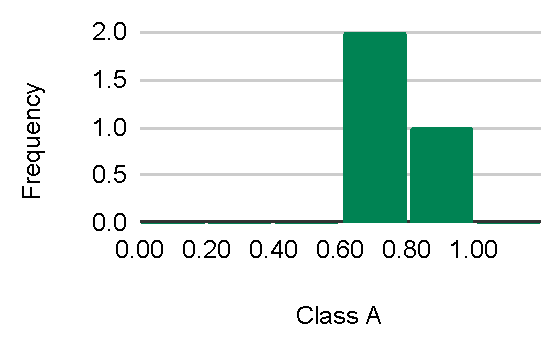
\includegraphics[width=\linewidth]{./Part I/ClassA.pdf}}}
        \subcaption{Histogram for Class A}
    \end{minipage}
    \hfill
    \begin{minipage}[t]{0.48\linewidth}
        \centering
        \resizebox{\linewidth}{!}{\fbox{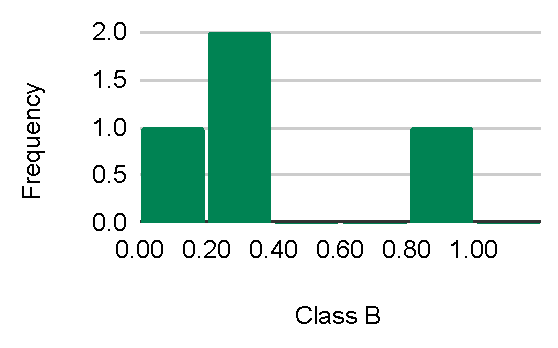
\includegraphics[width=\linewidth]{./Part I/ClassC.pdf}}}
        \subcaption{Histogram for Class B}
    \end{minipage}
    
    \vspace{0.5cm} 

    \begin{minipage}[t]{0.48\linewidth}
        \centering
        \resizebox{\linewidth}{!}{\fbox{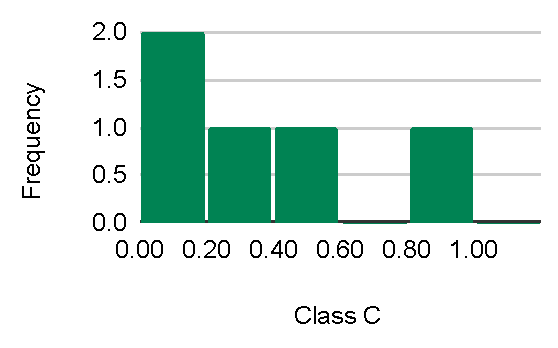
\includegraphics[width=\linewidth]{./Part I/ClassB.pdf}}}
        \subcaption{Histogram for Class C}
    \end{minipage}
    
    \caption{Class-conditional relative histograms of $y_1$ using 5 equal spaced bins in [0,1]}
\end{figure}

\vspace{15cm}

\item To find the root split using the discriminating rules for the empirical distributions, we draw a decision tree with just one root split on $y_1$.
Each branch contains the values of one bin, and it's corresponding leaf represents the class with highest value for that bin.
Since we are faced with a tie in branch $0.8 <= y_1 <= 1$, we will use the alphabetic ascending rule to make this decision (like in the first exercise).
\end{enumerate}

\begin{figure}[H]
    \centering
    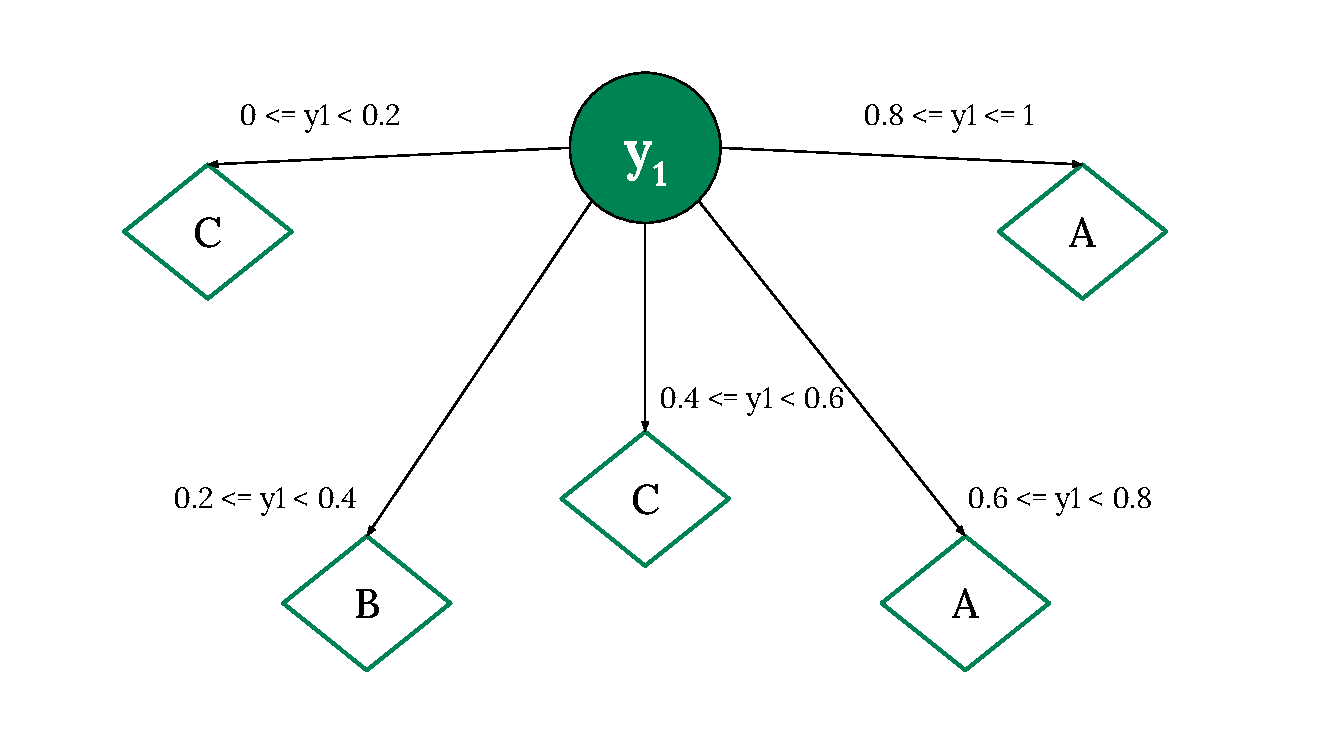
\includegraphics[width=15cm]{./Part I/5 ary root split.pdf}
    \caption{Decision Tree using the discriminant rules from the empirical distributions}
\end{figure}

\vspace{1cm}

\large{\textbf{Part II}: Programming}\normalsize

\vspace{1cm}

Consider the diabetes.arff data available at the homework tab, comprising 8 biological
features to classify 768 patients into 2 classes (normal, diabetes).

\vspace{0.5cm}

\begin{enumerate}[leftmargin=\labelsep,resume]
\setcounter{enumi}{0}
\item \textbf{ANOVA is a statistical test that can be used to assess the discriminative power of a
single input variable. Using f\_classif from sklearn, identify the input variables with the
worst and best discriminative power. Plot their class-conditional probability density
functions.}

\vspace{1cm}

\lstinputlisting[language=Python]{./Part II/1.py}

    \begin{figure}[H]
        \centering
          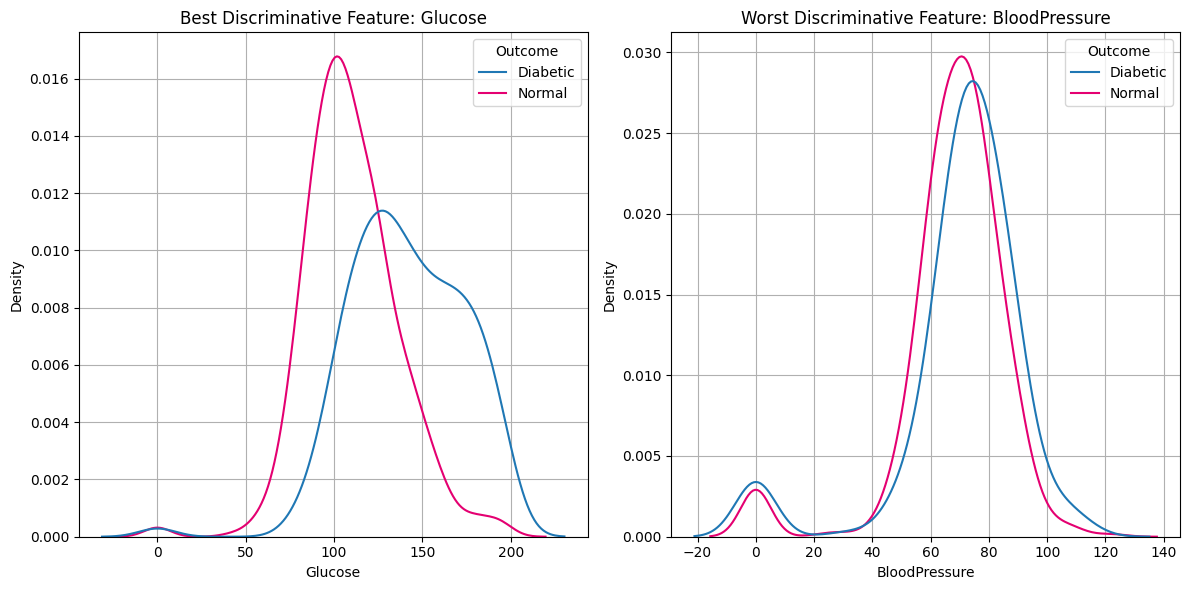
\includegraphics[width=12cm]{./Part II/1.png}
          \caption{Class-conditional probability density functions plot}
    \end{figure}

\vspace{2cm}

As we can see from the graphic above:
\begin{itemize}
    \item The variable with the best discriminative power is \textbf{Glucose}: It's visible that the distribution for `Diabetic' (blue line) has a significant shift compared to `Normal' (pink line), showing that glucose levels are a strong differentiating factor between the two classes.
    \item The variable with the worst discriminative power is \textbf{BloodPressure}: The distributions for both `Diabetic' and `Normal' classes overlap significantly, meaning this feature doesn't separate the two classes well.
\end{itemize}

\vspace{0.5cm}

\item \textbf{Using a stratified 80--20 training-testing split with a fixed seed (random\_state=1),
assess in a single plot both the training and testing accuracies of a decision tree with
minimum sample split in and the remaining parameters as default.}

\vspace{1cm}

\lstinputlisting[language=Python]{./Part II/2.py}

    \begin{figure}[H]
        \centering
          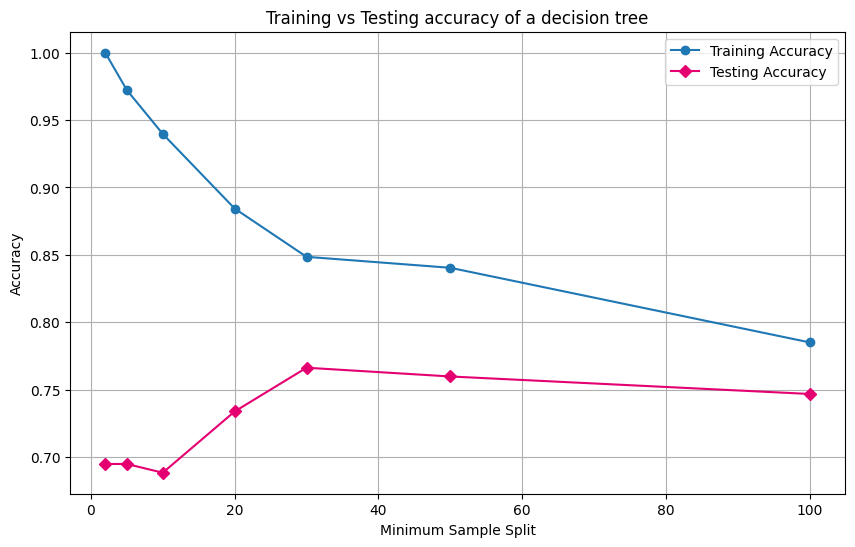
\includegraphics[width=12cm]{./Part II/2.png}
          \caption{Training and testing accuracies of a decision tree with various depth limits}
        \end{figure}

\vspace{0.5cm}

\item \textbf{Critically analyze these results, including the generalization capacity across settings}

\vspace{1cm}

As shown in the graph above, increasing the \texttt{min\_samples\_split} parameter leads to a roughly 20\% decrease in accuracy. This is expected because higher values of \texttt{min\_samples\_split} result in simpler trees, which reduces the model's ability to fit the training data accurately.

Regarding testing accuracy, we observe a slight initial decrease, indicating overfitting (high training accuracy but low testing accuracy). As \texttt{min\_samples\_split} increases, testing accuracy improves, reaching 75\%-80\%, which indicates better generalization. Beyond this point, testing accuracy slightly declines, suggesting the model is becoming underfit due to the tree's reduced complexity.

In terms of generalization, we can observe:

\begin{itemize}
    \item \textit{Underfitting} for higher \texttt{min\_samples\_split}, since both training and testing accuracy drop. This indicates the model is becoming too simplistic and fails to capture the underlying patterns in the data, leading to underfitting.
    
    \item Optimal generalization around 20--30 \texttt{min\_samples\_split}, where testing accuracy peaks, balancing bias and variance. The model complexity is reduced enough to avoid overfitting while retaining predictive power.
    
    \item Overfitting at Low \texttt{min\_samples\_split}, since The model fits the training data perfectly but performs poorly on test data, indicating poor generalization to new, unseen data.
\end{itemize}

The ideal minimal sample split appears to be around 30, which is the point in the graphic where the testing accuracy reaches its maximum, striking a balance between model complexity and generalization to new data. This would help us prevent the model from being too minimalistic (\textit{underfitting}) or overly complex (\textit{overfitting}).


\vspace{1cm}

\item \begin{flushleft}
    \textbf{To deploy the predictor, a healthcare provider opted to learn a single decision tree (random\_state=1) using all available data and ensuring 
that the maximum depth would be 3 in order to avoid overfitting risks.}
\end{flushleft}

\vspace{0.5cm}
    
    \textbf{(i) Plot the decision tree.} 

\lstinputlisting[language=Python]{./Part II/4.py}

    \begin{figure}[H]
        \centering
          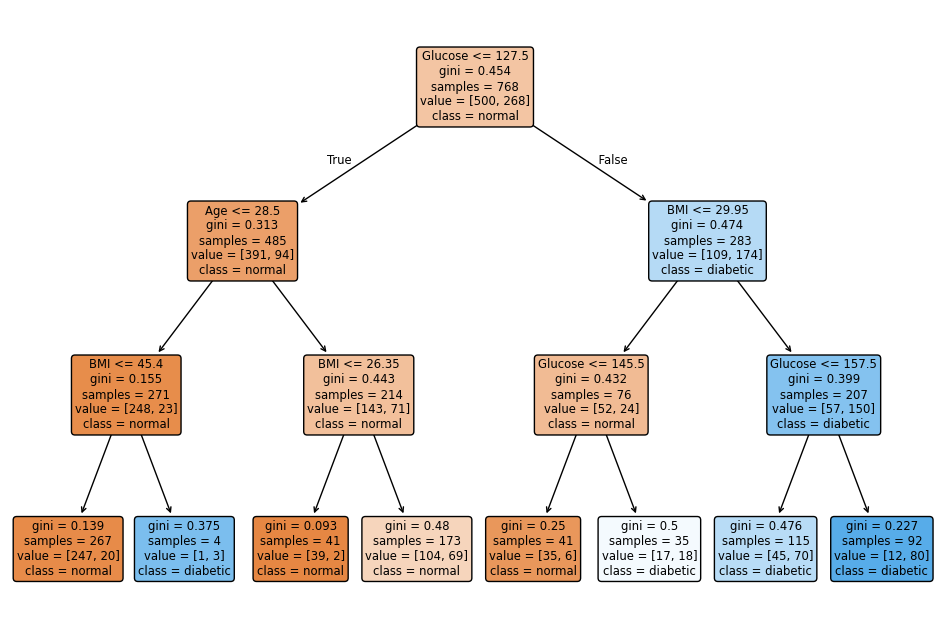
\includegraphics[width=15cm]{./Part II/4.png}
          \caption{Decision tree for exercise 4}
    \end{figure}

\vspace{2cm}

\textbf{(ii) Explain what characterizes diabetes by identifying the conditional associations
together with their posterior probabilities.}

The diabetic condition is characterized by:

\begin{itemize}
    \item Glucose $<= 127.5$, Age $<= 28.5$ and BMI $>= 45.4$
    \item Glucose $<= 127.5$ and BMI $>= 29.95$
\end{itemize}

The posterior probabilities are calculated using the following expression:

\[
PP = \frac{\text{node\_samples\_current\_class}}{\text{total\_node\_samples}}
\]

As we can see, the most critical features in determining diabetes are Glucose and BMI.\\ 
Glucose levels exceeding 127.5 significantly increase the likelihood of developing diabetes. For individuals with glucose levels surpassing 157.5, the posterior probability is $87\%$, indicating a high likelihood of suffering from a diabetic condition. 
Even with a lower BMI, high glucose levels still pose a considerable risk for diabetes. Specifically, a BMI above a certain threshold is strongly associated with an increased chance of being diabetic.


\end{enumerate}

\end{document}
